\documentclass[twoside]{article}
\setlength{\oddsidemargin}{0.25 in}
\setlength{\evensidemargin}{-0.25 in}
\setlength{\topmargin}{-0.6 in}
\setlength{\textwidth}{6.5 in}
\setlength{\textheight}{8.5 in}
\setlength{\headsep}{0.75 in}
\setlength{\parindent}{0 in}
\setlength{\parskip}{0.1 in}

\usepackage{graphicx}
\usepackage{url}

%
% The following commands sets up the lecnum (lecture number)
% counter and make various numbering schemes work relative
% to the lecture number.
%
\newcounter{lecnum}
\renewcommand{\thepage}{\thelecnum-\arabic{page}}
\renewcommand{\thesection}{\thelecnum.\arabic{section}}
\renewcommand{\theequation}{\thelecnum.\arabic{equation}}
\renewcommand{\thefigure}{\thelecnum.\arabic{figure}}
\renewcommand{\thetable}{\thelecnum.\arabic{table}}
\newcommand{\dnl}{\mbox{}\par}

%
% The following macro is used to generate the header.
%
\newcommand{\lecture}[4]{
  \pagestyle{myheadings}
  \thispagestyle{plain}
  \newpage
  \setcounter{lecnum}{#1}
  \setcounter{page}{1}
  \noindent
  \begin{center}
  \framebox{
     \vbox{\vspace{2mm}
   \hbox to 6.28in { {\bf COMPSCI~590S~~~Systems for Data Science
                       \hfill Fall 2017} }
      \vspace{4mm}
      \hbox to 6.28in { {\Large \hfill Lecture #1: #2  \hfill} }
      \vspace{2mm}
      \hbox to 6.28in { {\it Lecturer: #3 \hfill Scribe(s): #4} }
     \vspace{2mm}}
  }
  \end{center}
  \markboth{Lecture {#1}: #2}{Lecture {#1}: #2}
  \vspace*{4mm}
}

%
% Convention for citations is authors' initials followed by the year.
% For example, to cite a paper by Leighton and Maggs you would type
% \cite{LM89}, and to cite a paper by Strassen you would type \cite{S69}.
% (To avoid bibliography problems, for now we redefine the \cite command.)
%
\renewcommand{\cite}[1]{[#1]}

% \input{epsf}

%Use this command for a figure; it puts a figure in wherever you want it.
%usage: \fig{NUMBER}{FIGURE-SIZE}{CAPTION}{FILENAME}
\newcommand{\fig}[4]{
           \vspace{0.2 in}
           \setlength{\epsfxsize}{#2}
           \centerline{\epsfbox{#4}}
           \begin{center}
           Figure \thelecnum.#1:~#3
           \end{center}
   }

% Use these for theorems, lemmas, proofs, etc.
\newtheorem{theorem}{Theorem}[lecnum]
\newtheorem{lemma}[theorem]{Lemma}
\newtheorem{proposition}[theorem]{Proposition}
\newtheorem{claim}[theorem]{Claim}
\newtheorem{corollary}[theorem]{Corollary}
\newtheorem{definition}[theorem]{Definition}
\newenvironment{proof}{{\bf Proof:}}{\hfill\rule{2mm}{2mm}}

% Some useful equation alignment commands, borrowed from TeX
\makeatletter
\def\eqalign#1{\,\vcenter{\openup\jot\m@th
 \ialign{\strut\hfil$\displaystyle{##}$&$\displaystyle{{}##}$\hfil
     \crcr#1\crcr}}\,}
\def\eqalignno#1{\displ@y \tabskip\@centering
 \halign to\displaywidth{\hfil$\displaystyle{##}$\tabskip\z@skip
   &$\displaystyle{{}##}$\hfil\tabskip\@centering
   &\llap{$##$}\tabskip\z@skip\crcr
   #1\crcr}}
\def\leqalignno#1{\displ@y \tabskip\@centering
 \halign to\displaywidth{\hfil$\displaystyle{##}$\tabskip\z@skip
   &$\displaystyle{{}##}$\hfil\tabskip\@centering
   &\kern-\displaywidth\rlap{$##$}\tabskip\displaywidth\crcr
   #1\crcr}}
\makeatother

% **** IF YOU WANT TO DEFINE ADDITIONAL MACROS FOR YOURSELF, PUT THEM HERE:



% Some general latex examples and examples making use of the
% macros follow.

\begin{document}

%FILL IN THE RIGHT INFO.
%\lecture{**LECTURE-NUMBER**}{**DATE**}{**LECTURER**}{**SCRIBE**}
\lecture{13}{Bloom Filters and BigTable}{Emery Berger}{Abhiram Eshwaran, Akul Siddalingaswamy}

\section{Counting Bloom Filters (Continued)}

As discussed earlier, bloom filters are used for fast approximate lookup where we trade accuracy for space. Counting bloom filters are another variation which support deletion operation as well. 

Consider a sample bloom filter of 8 bits long [0 0 0 0 0 0 0 0] with 0-based indexing. Consider the operations of add(x), delete(x), ismember(x) where x is the input object. For now, let's take 2 strings- "foo" and "bar"

Also, consider 2 hash functions h\textsubscript{1}(x) and h\textsubscript{2}(x) which spit out the bit positions (one each) for the input x. Let's assume,\newline 
h\textsubscript{1}("foo") = 1 and h\textsubscript{2}("foo") = 2 \newline
h\textsubscript{1}("bar") = 2 and h\textsubscript{2}("bar") = 4 \newline

Initially, bloom = [0 0 0 0 0 0 0 0]\newline
add("foo") increments the bits at positions 1 and 2 by 1 making bloom = [0 1 1 0 0 0 0 0]\newline
Similarly, add("bar") increments the bits at positions 2 and 4 by 1 making bloom = [0 1 2 0 1 0 0 0]\newline
Now, if we execute ismember("foo"), we check positions 1 and 2. Since both are non-empty, the bloom filter outputs "MAYBE"\newline
Next, if we execute delete("foo"), we decrement the positions 1 and 2 by 1 making bloom = [0 0 1 0 1 0 0 0]\newline
However, if we now execute ismember("foo"), we check positions 1 and 2. Since both are empty, the bloom filter outputs "NO"\newline
This way, the counting bloom filter supports the delete operation.

\section{Web Search, Indexing and Spidering}

\subsection{A Primitive Web Search}
A simple Google query must crunch through petabyte of data to return the results of the query. There are two ways to do this,

\begin{itemize}
    \item Naive approach: Linear Search
    \item Better approach: Use indices to data, store this in Btree and this can be achieved in log time big O complexity.
\end{itemize}

But consider a query like ``Traffic In Boston For Friday'', this query will need to find an intersection of all results in Traffic, Boston and Friday to give the results. A perfect solution to the above problem would be an inverted index. 

\begin{figure}[h]
    \centering
  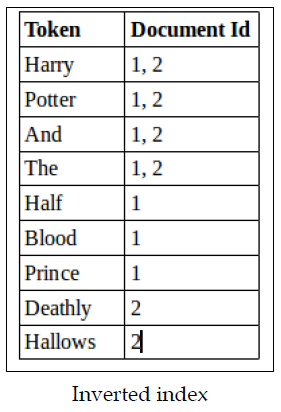
\includegraphics[scale=0.7]{images/iGri3.png}
  \caption{Inverted Index}
\end{figure}

\subsection{Inverted Index}
Consider the image above. Now a query like "Harry Potter and The Half Blood Prince" would take an intersection of all documents in the inverted index and return document 1 as the result.

But what if there are millions of results? The next challenge would be to order these millions of documents. This is know as \textbf{ranking}.

"\textbf{Link Span}" was one concept which determined the rank of a web page. If most results of a query pointed to a particular web page then that web page ended up getting a higher rank on the search results. This "link span" was later removed due to malicious websites exploiting this concept.

But we are still left with the task of creating a database for the web. This leads us to Spidering.

\subsection{Spidering}
We have the web, we have a spider, all we have to do now is crawl. So this what a web spider does. A web spider crawls the web. By crawl we mean, it takes a web page, get all the links in the web page and recursively follows all the links. (We use marking to prevent revisiting a web page)

The web spider crawls the web continuously. Pages are cached with different frequencies and this is done really fast. (Google News leverages this to present all the breaking news). Few important characteristics of the web spider,

\begin{itemize}
\item Needs to store only the most recent version.
\item The Web Spider is basically just writes. Writes need to be super efficient and new versions should be managed.
\item Disk storage is crucial. Seek time for random access is a pain and the memory has to be defragmented. We solve this particular problem by GFS which does only bulk writes.
\end{itemize}

\section{BigTable}
\subsection{Motivation for BigTable}
As discussed above, periodic crawling could help keep the pages up-to date. However, if there are millions of pages, it becomes expensive to do these writes/updates one at a time (seek time + rotational latency + transfer time for each write). A solution to this is to just write sequentially in the form of a log, a.k.a Log-Structured File System. Write throughput on optical and magnetic disks improves because the writes can be batched into large sequential runs and costly seeks are kept to a minimum. However, when we try to read them, we hit a bottleneck since the data is sequential. As a way of providing random access to the data, an index is created for this log-structured file system and this index is basically BigTable.

\subsection{Data model}
Generally, NoSQL datadases store data as simple \textit{key} $\,\to\,$ \textit{value} pairs. Bigtable's data model is a generalization of such data storage systems. Here, the map is indexed by a row key, column key, and a timestamp: \textit{(row:string, column:string, time:int64)} $\,\to\,$ \textit{(value:string)}\\


\begin{tabular}{|c|c|c|c||c|}
\hline
Column1 & Column2 & ... & ColumnN & Value \\
\hline
        &         &     &         &       \\
\hline
        &         &     &         &       \\
\hline
        &         &     &         &       \\
\hline
\end{tabular}
A logical overview of Bigtable rows

A general way of key-value stores is to map all the columns to a single row key. But BigTable key is a triple where they have (row, column, timestamp) and allow accessing a column directly. Bigtable is a dense data store, which means it has cells with non-empty data. Using timestamps, different versions of a cell are maintained in most-recent-first order. The number of versions depend on a threshold set that specifies only the last \textit{n} versions of a cell be kept. The columns are grouped as families, and each column is identified as a pair \textit{(family: qualifier)}. The row IDs are sorted and split into different groups called \textit{tablets}. This lets BigTable take advantage of locality of data.

\begin{figure}[h]
\centering
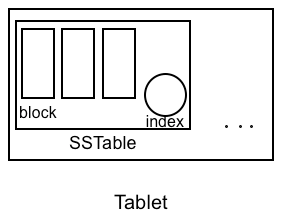
\includegraphics[width=0.5\linewidth]{images/tablet.png}
\caption[]{Tablet structure}
\end{figure}

\subsection{Tablet}
Each tablet contains one or more SSTables. SSTable (Sorted String Table) is a file format that provides an immutable, ordered key-value map. An SSTable contains multiple blocks (or chunks) and an index to locate the blocks. SSTables use binary search within the block for finding rows. Additionally, the recently committed updates are stored in memory in a sorted buffer called \textit{memtable}. When the memtable size reaches a threshold, it is frozen and converted to an SSTable. 

\end{document}
